\documentclass{article}
\usepackage[utf8]{inputenc}

\title{LegendOfBluespec}
\author{kr469 }
\date{October 2021}

\begin{document}

\maketitle

\section{Core loop of Bluespec}
    In Bluespec all computation is done in form of rules. Each cycle we will take a subset of all rules that we are going to execute in this cycle, rule is fired (executed) in cycle only if it's ready (or will be ready) and it's not conflicting with other rules (If this happens compiler must issue a warning, and picks arbitrary rule to fire from subset of conflicting rules). Each rule can fire at most one time per cycle. For rule to be ready to fire it needs it's implicit and explicit conditions to be true. Rule can be fired in a cycle even if it's not ready at the start of cycle, for example if you add item on an empty queue and then pop can happen in same cycle.
    %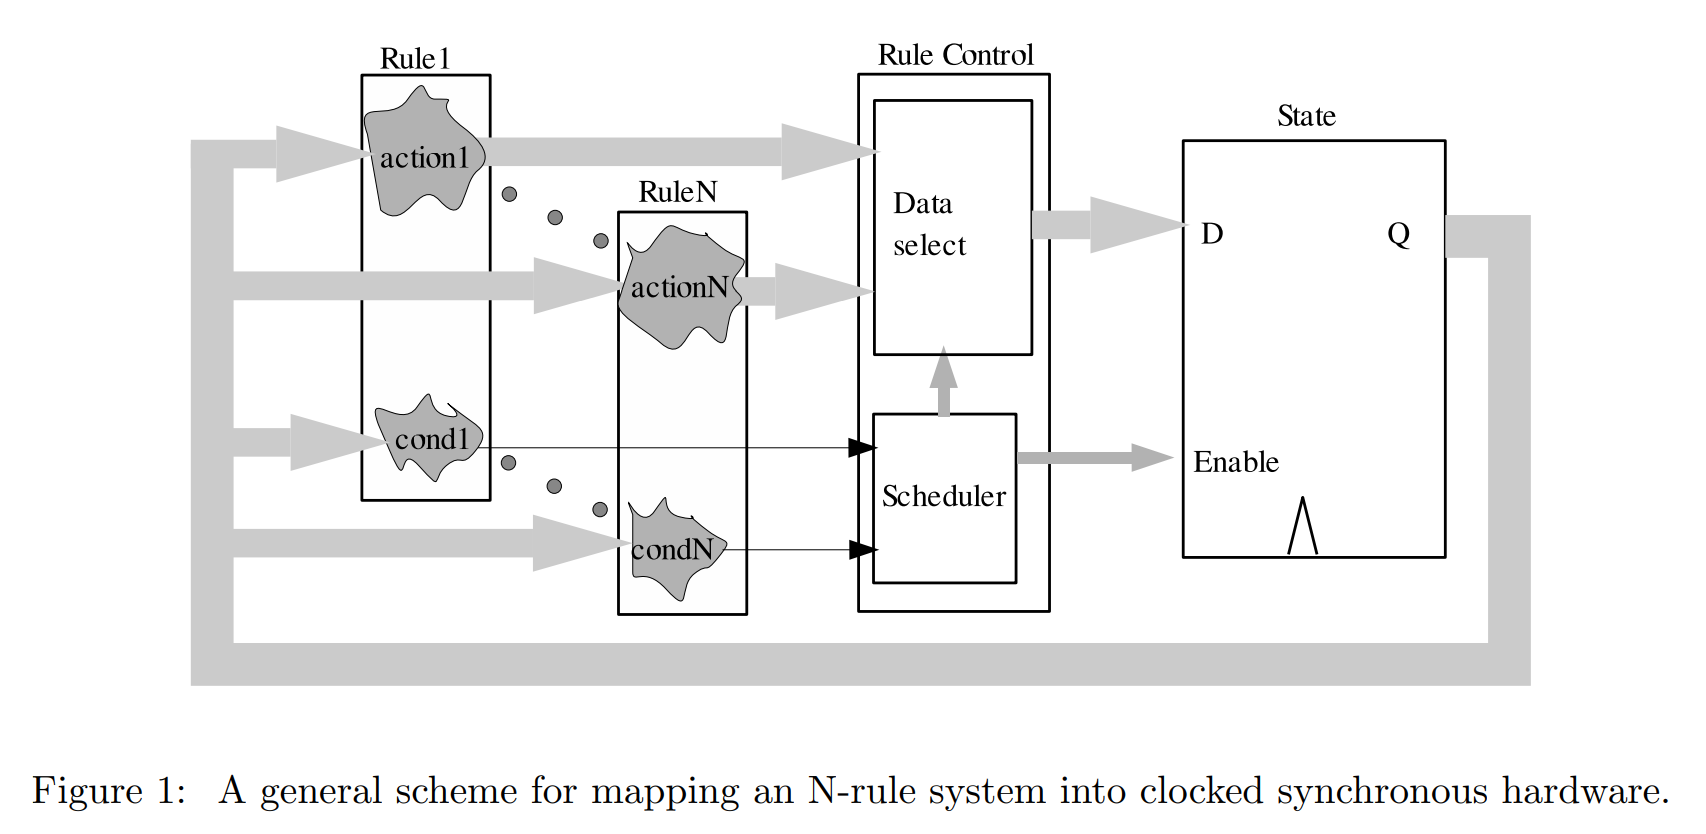
\includegraphics[]{Rulemapping.png}
    \begin{verbatim}
        
        TODO: piece of Bluespec with module using fifo and other rule explaining types of conditions.
        
    \end{verbatim}

\section{Types}
    I'm not sure how long this section need to be so I'm going to leave it for later. Idea of this section is to talk about that there are things like numeral types that are not synsesiable by definition.
    In Bluespec we can enounter types in 4 categories:
    \subsection{Bit Types}
        This is most common category and contains evey type that is ment to represent data like Int, Bit , Tuples. They are synthesiazable and can store data.
    \subsection{Non-Bit types}
        Those are things like Integer, Real , String that are ment to be used for debug or polymorphism therefore making it easy to tell wheather you can do computations on them at runtime. 
    \subsection{Interface types}
        This set of types are ment to represent implementation independed sets of functions exposed by a module.
    \subsection{Compiler types}
        Those are things like Action, ActionValue,Rules which are more of a keywords rather than types, and they are used by compiler do distinguish functions that are Rules(they can't be called), from Actions which can be called.
    

\section{Interfaces}
    In Bluespec all modules need to have interfaces. Those interfaces provide a framework for communication between modules. They are like a structs that contains only methods or sub stucts. Interfaces can be polymorphic and we will use this fact to create interfaces that allow for translation between interfaces. A common example would be polymorphic FIFO that can store any type. What's important is that this polymorphism makes it insyntesiable and it's exact type needs to be resolved before module with such type can be synthesied.
    \\
    TODO : I might add grammar for defining an interface from reference guide.  
    
\section{Methods or rather actions}
    I will fill this section later, it's going to be about distinction about Action , Value methods.
\section{Provisios}
    I will add some side note on provisos, and why handling them would require compilation of bluespec, and that I will check them via running bluespec compiler with some dummpy instantiating of module.
    
\section{Bluectl}
    Here I will explain what can be extracted from Bluectl.
    For me most important will be extracting interfaces and functions for module creation.
    To do this I have written down grammar (it's currently in type.lark but I will paste it at some point here).
    
\section{GetPut and other libraries}
    GetPut is library used to make it easier to connect modules,
    but because it is written using normal type system it therore it should be possibe to generalize and handle them via main algorithm without special exception.

\section{System Verilog}
    Using respecticive complier flags one can complie Bluespec to verilog and one can add verilog inserts into bluespec. Because of this I will focus only on support for bluespec as there is avaliable tooling to make my tools work in verilog projects with bluespec inserts.

\

\end{document}
